
Experiments evaluating the performance of the set of FVR related algorithms on active sensor camera input are presented here. These data sets are all 24-25 frames long and captured different environments using different camera movements. Due to the limitations of the Asus Xtion Pro Live active camera used, primarily indoor scenes were captured. Similar to the results presented in section \ref{StereoSOTA}, statistics are presented for algorithms from the literature (FM2D, FM3D, ICP and PCA) as well as FVR based algorithms (FVR, FFVR and FVR-3D) in the form of the median registration error and the percentage of best results. Raw frame registration errors are presented in Appendix \ref{ActiveResultsRaw}. \\

All test data were generated using the Asus Xtion Pro Live camera. Each scene was captured using a specific type of camera movement. Some scenes were captured by rotating the camera about the x or y-axis, others by translating the camera. By testing with different movements, future algorithms may be constructed by switching to different registration methods based on camera movement. Additionally, a difficult scene containing areas prone to texture confusion was captured. \\

The first scene, the Apartment Texture Rotate scene, was taken by rotating the camera around the y-axis across an apartment. This scene contains a lot of texture information. The Apartment Texture X Axis Rotation scene is similar in terms of texture but contains x-axis rotation rather than y axis rotation. These different scenes test each method's ability to register 3D pose. The Office Textured Blind-spot Rotation scene is a textured office scene where the camera is rotated about the y-axis. The scene is focused on a large divider which separates two desks. The divider may confuse registration methods which rely too heavily on minimization by aligning the large divider as a priority rather than taking into account the smaller details within the scene. An example of such an algorithm would be ICP and its derivatives. An Office Textured Items Translation and an Office Texture Rotation data set are also captured. These office scenes are standard and contain fair amounts of texture. Another scene, Parks, Plants and Table, was captured by translating and rotating the camera across a scene with plenty of texture confusion.  \\




Table \ref{tab:apartmenttexturerotate} shows results for the Apartment Texture Rotation Data Set, Figure \ref{fig:Apartment_Texture_rotate} shows some example RGB image frames. The scene filled in these data frames are of an apartment living room, where the camera is rotated approximately 90 degrees over 25 frames. The scene contains an abundance of texture information. Results show that the FVR-3D method achieved the lowest median error result, making it the top performer in terms of this metric. FM2D performed next best, followed by the FVR method. The FVR algorithm outperformed all other algorithms except FVR-3D and FM2D on this data set. In terms of the percentage of best results metric, FVR-3D achieved the highest percentage at 36 \%, FM2D was second at ~28 \%. A hybrid FVR method would have produced a 60\% record of achieving the best registration result on these frames. \\

%%Apartment Texture Rotate:
\begin{table}[t]
\centering
\caption{Reconstruction Errors for the Apartment Texture Rotate Data Set}
\begin{tabular}{ccc}
\hline
\textbf{Algorithm} & \textbf{Median Error $\times$ 1000} & \textbf{\% best results}\\ \hline
FM2D	& 2.13 & 28\%\\
FM3D	& 5.14 & 0\%\\
ICP	& 2.42 & 8\%\\
PCA	& 8.61 & 4\%\\
FVR	& 2.26 & 16\%\\
FFVR	& 2.7 & 8\%\\
FVR-3D	& 2 & 36\%\\
\end{tabular}
\label{tab:apartmenttexturerotate}
\end{table} 

%apartment_texture_rotate
\begin{figure*}[t]
\centering
\begin{subfigure}[b]{6.8cm}
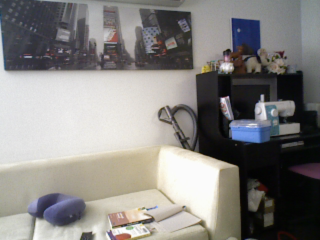
\includegraphics[width=6.5cm]{{images/experiments/test_data/Apartment.Texture.rotate.0}.png}
\caption{Frame 1}
\end{subfigure}%
\begin{subfigure}[b]{6.8cm}
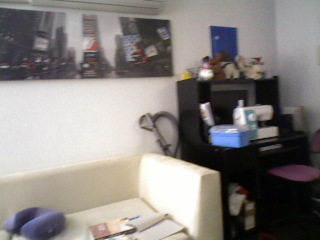
\includegraphics[width=6.5cm]{{images/experiments/test_data/Apartment.Texture.rotate.1}.png}
\caption{Frame 10}
\end{subfigure}
\begin{subfigure}[b]{6.8cm}
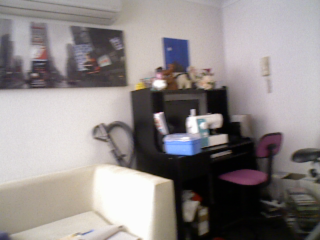
\includegraphics[width=6.5cm]{{images/experiments/test_data/Apartment.Texture.rotate.2}.png}
\caption{Frame 15}
\end{subfigure}%
\begin{subfigure}[b]{6.8cm}
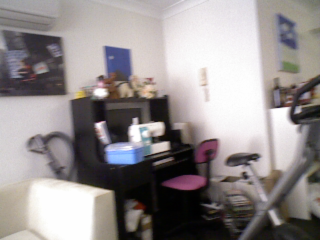
\includegraphics[width=6.5cm]{{images/experiments/test_data/Apartment.Texture.rotate.3}.png}
\caption{Frame 20}
\end{subfigure}%
\caption{Four Sample Frames from the Apartment Texture Rotate Data Set}
\label{fig:Apartment_Texture_rotate}
\end{figure*}



Results for the Apartment Texture X-Axis Rotation Data Set are presented in Table \ref{tab:apartmenttexturex-axisrotation}. Figure \ref{fig:Apartment_Texture_rotateXAxis} shows some example image frames of this data set. This scene was captured by rotating the Asus Xtion Pro Live active camera about the x-axis. The scene contains a Christmas tree as well as some bags on the floor in the centre of an apartment room and some chairs to the right of the frame. Out of the set of FVR based techniques, only FVR-3D is capable of full 3D rotation registration, FVR and FFVR are only capable of being robust to this type of registration (handling it in the best way possible using translation, scaling and y-axis rotational transforms). Results show that the ICP method achieved the lowest median registration error with FVR-3D achieving the second best result. In terms of the percentage of best results metric, FVR-3D outperformed ICP and the others 64 \% of the time compared to ICP at 28 \%. Interestingly, both FVR and FFVR outperformed PCA and FM3D despite these methods' abilities to register full 3D rotation (including x-axis). In terms of the percentage of best match metric, the set of FVR algorithms outperformed the others around 68 \% of the time. \\

%%Apartment Texture X-Axis Rotation
\begin{table}[t]
\centering
\caption{Reconstruction Errors for the Apartment Texture X-Axis Rotation Data Set}
\begin{tabular}{ccc}
\hline
\textbf{Algorithm} & \textbf{Median Error $\times$ 1000} & \textbf{\% best results}\\ \hline
FM2D	& 1.97 & 4\%\\
FM3D	& 2.58 & 0\%\\
ICP	& 1.78 & 28\%\\
PCA	& 3.81 & 0\%\\
FVR	& 1.99 & 4\%\\
FFVR	& 2.01 & 0\%\\
FVR-3D	& 1.82 & 64\%\\
\end{tabular}
\label{tab:apartmenttexturex-axisrotation}
\end{table} 

%apartment_texture_rotateX_axis
\begin{figure*}[t]
\centering
\begin{subfigure}[b]{6.8cm}
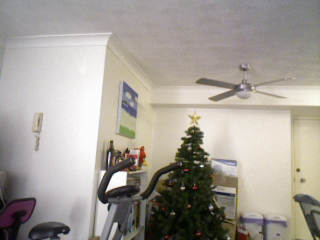
\includegraphics[width=6.5cm]{{images/experiments/test_data/Apartment.Texture.rotateXAxis.0}.png}
\caption{Frame 1}
\end{subfigure}%
\begin{subfigure}[b]{6.8cm}
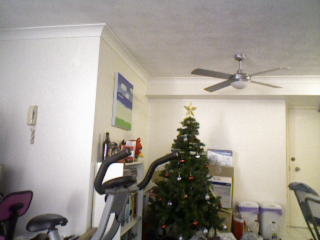
\includegraphics[width=6.5cm]{{images/experiments/test_data/Apartment.Texture.rotateXAxis.1}.png}
\caption{Frame 10}
\end{subfigure}
\begin{subfigure}[b]{6.8cm}
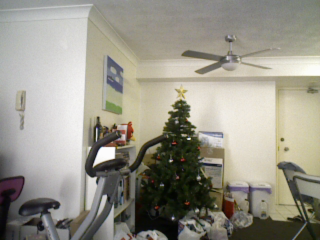
\includegraphics[width=6.5cm]{{images/experiments/test_data/Apartment.Texture.rotateXAxis.2}.png}
\caption{Frame 15}
\end{subfigure}%
\begin{subfigure}[b]{6.8cm}
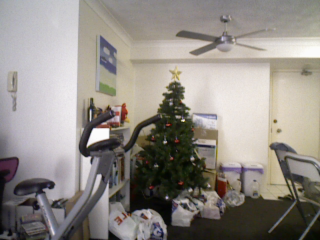
\includegraphics[width=6.5cm]{{images/experiments/test_data/Apartment.Texture.rotateXAxis.3}.png}
\caption{Frame 20}
\end{subfigure}%
\caption{Four Sample Frames from the Apartment Texture X-Axis Rotation Data Set.}
\label{fig:Apartment_Texture_rotateXAxis}
\end{figure*}



Table \ref{tab:desktexturetranslation} shows the results for the Desk Texture Translation scene, Figure \ref{fig:Desk_Texture_Translation} shows some example image frames for this data set. This scene includes a desk, a computer and computer monitor as well as several items including books, a hat and pair of glasses. The scene was captured by moving the Asus Xtion Pro Live active camera directly down the x-axis to the right in a purely translational movement. Results show that the FVR-3D method achieved the lowest median registration error, with ICP performing second best. In this test, the FVR method outperformed the others in terms of median registration error. This is likely due to the fact that the camera was moved in a purely translational way compared to previous tests. The next lowest median error value was achieved by the FVR-3D algorithm, followed by FM2D. Interestingly in the percentage of best results metric, ICP, which achieved a higher median error than all algorithms except FM3D, had the highest individual percentage of best results value of 28 \%. Combined, the FVR, FVR-3D and FFVR methods achieved the best frame registration around 48 \% of the time.

%% desk texture translation
\begin{table}[t]
\centering
\caption{Reconstruction Errors for the Desk Texture Translation Data Set}
\begin{tabular}{ccc}
\hline
\textbf{Algorithm} & \textbf{Median Error $\times$ 1000} & \textbf{\% best results}\\ \hline
FM2D	& 1.24 & 8\%\\
FM3D	& 2.48 & 12\%\\
ICP	& 1.59 & 28\%\\
PCA	& 1.51 & 4\%\\
FVR	& 1.16 & 16\%\\
FFVR	& 1.29 & 16\%\\
FVR-3D	& 1.23 & 16\%\\
\end{tabular}
\label{tab:desktexturetranslation}
\end{table} 

%desk_texture_translation
\begin{figure*}[t]
\centering
\begin{subfigure}[b]{6.8cm}
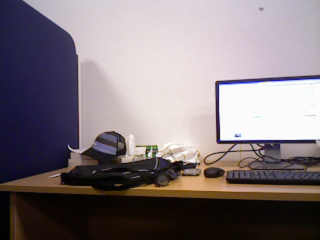
\includegraphics[width=6.5cm]{{images/experiments/test_data/Desk.Texture.Translation.0}.png}
\caption{Frame 1}
\end{subfigure}%
\begin{subfigure}[b]{6.8cm}
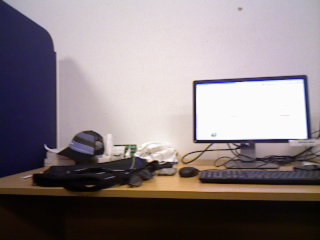
\includegraphics[width=6.5cm]{{images/experiments/test_data/Desk.Texture.Translation.1}.png}
\caption{Frame 10}
\end{subfigure}
\begin{subfigure}[b]{6.8cm}
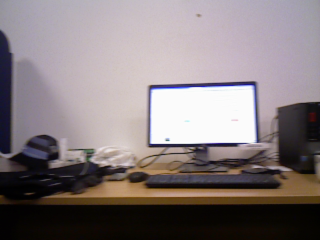
\includegraphics[width=6.5cm]{{images/experiments/test_data/Desk.Texture.Translation.2}.png}
\caption{Frame 15}
\end{subfigure}%
\begin{subfigure}[b]{6.8cm}
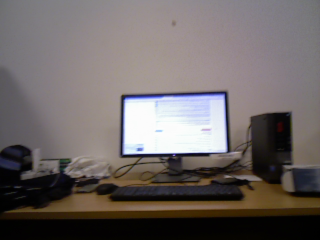
\includegraphics[width=6.5cm]{{images/experiments/test_data/Desk.Texture.Translation.3}.png}
\caption{Frame 20}
\end{subfigure}%
\caption{Four Sample Frames from the Desk Texture Translation Data Set.}
\label{fig:Desk_Texture_Translation}
\end{figure*}




Table \ref{tab:officetexturedblindspotrotation} shows the results for the Office Textured Blind-spot Rotation data set. Figure \ref{fig:Office_Texture_blindSpotRotation} shows some example frames from this data set. The scene is identical to the previous one (results presented in Table \ref{tab:desktexturetranslation}, but the camera was rotated about the y-axis rather than translated about the x-axis). The scene contains a large blind-spot in which a part of the scene is hidden by a divider, the effect of which was to intentionally reduce overlap in terms of frame registration making it more difficult for these algorithms to compute registration accurately. Results show that the FVR-3D method achieved the lowest median error, but tied in second place with FM2D in terms of percentage of best results. In this data set, ICP achieved the highest percentage of best results. \\

%%Office Textured Blindspot Rotation
\begin{table}[t]
\centering
\caption{Reconstruction Errors for the Office Texture Blind-spot Rotation Data Set}
\begin{tabular}{ccc}
\hline
\textbf{Algorithm} & \textbf{Median Error $\times$ 1000} & \textbf{\% best results}\\ \hline
FM2D	& 1.39 & 24\%\\
FM3D	& 5.92 & 0\%\\
ICP	& 1.2 & 44\%\\
PCA	& 4.83 & 8\%\\
FVR	& 2.07 & 0\%\\
FFVR	& 2.92 & 0\%\\
FVR-3D	& 1.1 & 24\%\\
\end{tabular}
\label{tab:officetexturedblindspotrotation}
\end{table} 

%office_texture_blindspotrotation
\begin{figure*}[t]
\centering
\begin{subfigure}[b]{6.8cm}
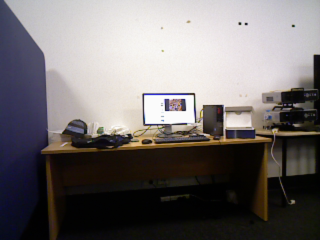
\includegraphics[width=6.5cm]{{images/experiments/test_data/Office.Texture.blindSpotRotation.0}.png}
\caption{Frame 1}
\end{subfigure}%
\begin{subfigure}[b]{6.8cm}
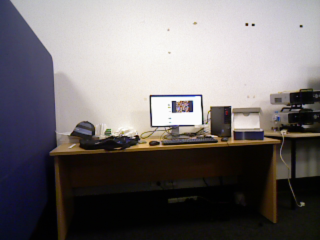
\includegraphics[width=6.5cm]{{images/experiments/test_data/Office.Texture.blindSpotRotation.1}.png}
\caption{Frame 10}
\end{subfigure}
\begin{subfigure}[b]{6.8cm}
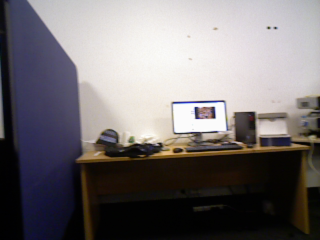
\includegraphics[width=6.5cm]{{images/experiments/test_data/Office.Texture.blindSpotRotation.2}.png}
\caption{Frame 15}
\end{subfigure}%
\begin{subfigure}[b]{6.8cm}
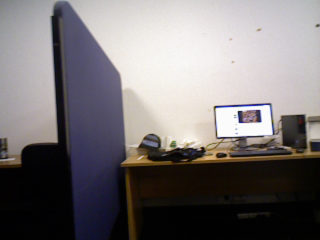
\includegraphics[width=6.5cm]{{images/experiments/test_data/Office.Texture.blindSpotRotation.3}.png}
\caption{Frame 20}
\end{subfigure}%
\caption{Four Sample Frames from the Office Textured Blind-spot Rotation Data Set.}
\label{fig:Office_Texture_blindSpotRotation}
\end{figure*}



Table \ref{tab:officetextureditemstranslation} presents results for the Office Textured Items Translation Data Set, whilst figure \ref{fig:Office_TexturedItems_Translation} shows some example captured frames. This scene was captured of a large room with large pieces of furniture, a large screen and a set of desks and chairs. This is another scene in which x-axis translation was the primary camera movement. Results show that the FVR-3D algorithm achieved both the lowest median error and the highest percentage of best results. Combined, the FVR methods achieved the best result ~72\% of the time. After FVR-3D and FFVR, FM2D performed next best with the second lowest median error score and 3rd highest percentage of best result score. \\

%%Office Textured Items Translation
\begin{table}[t]
\centering
\caption{Reconstruction Errors for the Office Textured Items Translation Data Set}
\begin{tabular}{ccc}
\hline
\textbf{Algorithm} & \textbf{Median Error $\times$ 1000} & \textbf{\% best results}\\ \hline
FM2D	& 2.89 & 24\%\\
FM3D	& 5.45 & 0\%\\
ICP	& 2.93 & 4\%\\
PCA	& 3.79 & 0\%\\
FVR	& 5.04 & 0\%\\
FFVR	& 3.06 & 28\%\\
FVR-3D	& 2.83 & 44\%\\
\end{tabular}
\label{tab:officetextureditemstranslation}
\end{table} 

%office_textured_items_translation
\begin{figure*}[t]
\centering
\begin{subfigure}[b]{6.8cm}
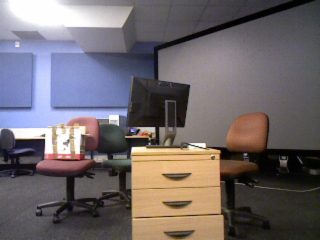
\includegraphics[width=6.5cm]{{images/experiments/test_data/Office.TexturedItems.Translation.0}.png}
\caption{Frame 1}
\end{subfigure}%
\begin{subfigure}[b]{6.8cm}
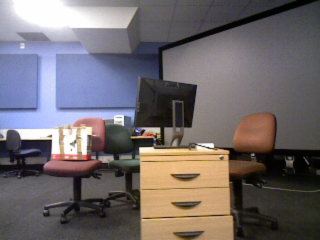
\includegraphics[width=6.5cm]{{images/experiments/test_data/Office.TexturedItems.Translation.1}.png}
\caption{Frame 10}
\end{subfigure}
\begin{subfigure}[b]{6.8cm}
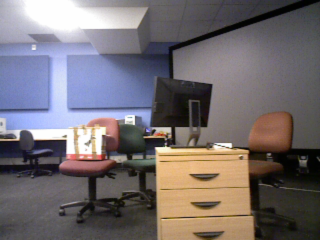
\includegraphics[width=6.5cm]{{images/experiments/test_data/Office.TexturedItems.Translation.2}.png}
\caption{Frame 15}
\end{subfigure}%
\begin{subfigure}[b]{6.8cm}
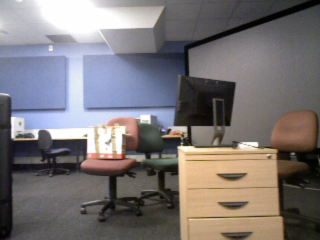
\includegraphics[width=6.5cm]{{images/experiments/test_data/Office.TexturedItems.Translation.3}.png}
\caption{Frame 20}
\end{subfigure}%
\caption{Four Sample Frames from the Office Textured Items Translation Data Set.}
\label{fig:Office_TexturedItems_Translation}
\end{figure*}


Table \ref{tab:parkplantsandtables} presents results for the Park Plants and Tables Rotation Data Set, Figure \ref{fig:parksplantandtable} shows some example frames from the data set. The scene captured was of an outdoors park area. In the scene, there is a metal table and metal fence surrounding a dense garden. This type of scene was expected to cause large amounts of texture confusion, as the metal fence and interspersed sections of garden appear to be similar locally. The primary camera movements were translation and y-axis rotation. Results are interesting and show that FM2D, FM3D and PCA were thrown off by this texture confusion. In terms of both median error and percentage of best result, the FVR method beat all other algorithms 76 \% of the time, and had the lowest median error score. ICP performed next best, followed by FVR-3D. A hybrid FVR based method would have produced the best result 84 \% of the time. \\



%parks plants and tables
\begin{table}[t]
\centering
\caption{Reconstruction Errors for the Park, Plants and Tables Rotation Data Set}
\begin{tabular}{ccc}
\hline
\textbf{Algorithm} & \textbf{Median Error $\times$ 1000} & \textbf{\% best results}\\ \hline
FM2D	& 10.2 & 4\%\\
FM3D	& 19.7 & 0\%\\
ICP	& 15.03 & 12\%\\
PCA	& 24 & 0\%\\
FVR	& 8.03 & 76\%\\
FFVR	& 16.47 & 0\%\\
FVR-3D	& 19.4 & 8\%\\
\end{tabular}
\label{tab:parkplantsandtables}
\end{table} 

%park.plants.and.tables
\begin{figure*}[t]
\centering
\begin{subfigure}[b]{6.8cm}
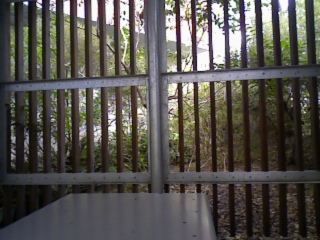
\includegraphics[width=6.5cm]{{images/experiments/test_data/PlantsOutdoors.tc.rotation.0}.png}
\caption{Frame 1}
\end{subfigure}%
\begin{subfigure}[b]{6.8cm}
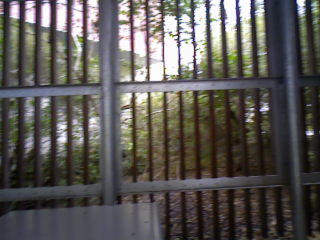
\includegraphics[width=6.5cm]{{images/experiments/test_data/PlantsOutdoors.tc.rotation.1}.png}
\caption{Frame 10}
\end{subfigure}
\begin{subfigure}[b]{6.8cm}
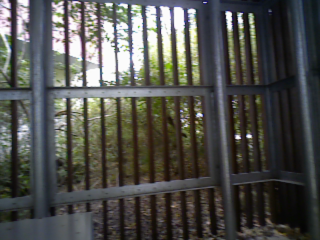
\includegraphics[width=6.5cm]{{images/experiments/test_data/PlantsOutdoors.tc.rotation.2}.png}
\caption{Frame 15}
\end{subfigure}%
\begin{subfigure}[b]{6.8cm}
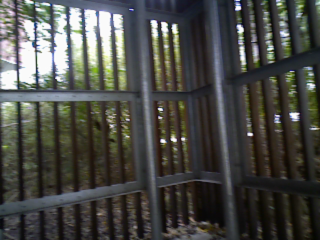
\includegraphics[width=6.5cm]{{images/experiments/test_data/PlantsOutdoors.tc.rotation.3}.png}
\caption{Frame 20}
\end{subfigure}%
\caption{Four Sample Frames from the Park Plants and Table Data Set.}
\label{fig:parksplantandtable}
\end{figure*}




In the final experiment using the Asus Xtion Pro Live Active sensor camera, another large office space was filmed with y-axis rotation being the primary camera movement, some example frames are shown in Figure \ref{fig:Office_Texture_rotation}. This scene was named the Office Texture Rotation Data Set and statistics for the registration results are presented in Table \ref{tab:officetexturerotation}. These results reveal the FVR-3D method achieved the lowest median error result but only the third highest percentage of best results score. A hybrid FVR based method would have achieved the best result around 38.46 \% of the time. In terms of median error, FM2D was better than ICP but their positions were reversed in the percentage of best results metric. 

%%office texture rotation
\begin{table}[t]
\centering
\caption{Reconstruction Errors for the Office Texture Rotation Data Set}
\begin{tabular}{ccc}
\hline
\textbf{Algorithm} & \textbf{Median Error $\times$ 1000} & \textbf{\% best results}\\ \hline
FM2D	& 4.36 & 26.92\%\\
FM3D	& 7.15 & 0\%\\
ICP	& 4.76 & 34.62\%\\
PCA	& 6.55 & 0\%\\
FVR	& 5.3 & 7.69\%\\
FFVR	& 4.74 & 7.69\%\\
FVR-3D	& 4.35 & 23.08\%\\
\end{tabular}
\label{tab:officetexturerotation}
\end{table} 

%office_texture_rotation
\begin{figure*}[t]
\centering
\begin{subfigure}[b]{6.8cm}
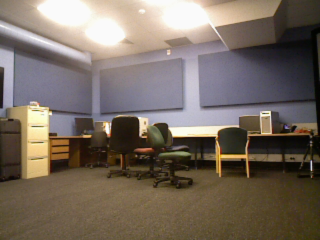
\includegraphics[width=6.5cm]{{images/experiments/test_data/Office.Texture.rotation.0}.png}
\caption{Frame 1}
\end{subfigure}%
\begin{subfigure}[b]{6.8cm}
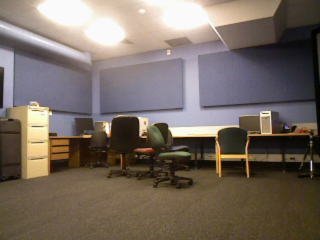
\includegraphics[width=6.5cm]{{images/experiments/test_data/Office.Texture.rotation.1}.png}
\caption{Frame 10}
\end{subfigure}
\begin{subfigure}[b]{6.8cm}
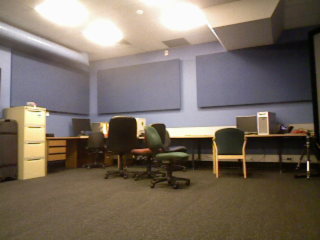
\includegraphics[width=6.5cm]{{images/experiments/test_data/Office.Texture.rotation.2}.png}
\caption{Frame 15}
\end{subfigure}%
\begin{subfigure}[b]{6.8cm}
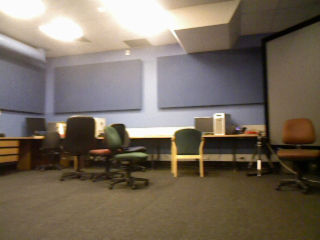
\includegraphics[width=6.5cm]{{images/experiments/test_data/Office.Texture.rotation.3}.png}
\caption{Frame 20}
\end{subfigure}%
\caption{Four Sample Frames from the Office Texture Rotation Data Set.}
\label{fig:Office_Texture_rotation}
\end{figure*}
